\documentclass[relatorio.tex]{subfiles}
\begin{document}
    
\subsection{\textit{Bezier Patches}} \label{subsec:bezier_p}

A construção das superfícies 3D foi dificultada por uma confusão das curvas a desenhar. 
Inicialmente, os \textit{patches} estavam a ser construídos a partir da estratégia de \textit{Catmull-Rom} e
dado a ser com base num \textit{line loop}, não estavam a ser desenhados triângulos, logo o bule final estava longe da representação desejada.
Para além disso, não estavam a ser desenhadas as divisões corretas com base no \textbf{nível de tesselação}, como em \textit{bezier patches},
só estavam a ser desenhados mais segmentos na curva.

Neste sentido, após uma análise do material fornecido pela equipa docente foram construídas 3 classes para permitir definir os triângulos das superfícies:
\begin{itemize}
    \item \mintinline{cpp}{class Matrix}
    \item \mintinline{cpp}{class PointMatrix}
    \item \mintinline{cpp}{class BezierTriangles}
\end{itemize}

\subsubsection{Classe Matrix}
Envés de representar as matrizes como apontadores para valores, como foi o caso das aulas práticas,
procurou-se definir um módulo que facilmente representaria uma matriz. 
\begin{code}
    \captionof{listing}{Matrix}
    \label{code:matrix.h}
    \inputminted[firstline=14, lastline=19]{cpp}{../../cartesian/matrix.h}
\end{code}

Deste modo, de forma encapsulada encontram-se na classe todas as operações relativamente a uma matriz e entre matrizes.
Não obstante a possibilidade de \textbf{transpor} e \textbf{clonar} uma matriz, foi definida a multiplicação entre a matriz local e outra; 
como a matriz local pode encontrar-se antes ou depois, recorreu-se ao \textbf{polimorfismo} da linguagem para construir os dois métodos 
considerando as possibilidades.
Para a classe foram criados diversos construtores, para inicializar a matriz, sendo um deles respetivo à construção das matrizes 
de transformação para os tipos de curva a serem usados:
\begin{code}
    \captionof{listing}{Matrix}
    \label{code:matrix.h}
    \inputminted[firstline=7, lastline=12]{cpp}{../../cartesian/matrix.h}
\end{code}
\dots como são sempre estáticos facilita o grupo ao usá-los nos cálculos dos pontos de uma curvas.

\subsubsection{Class PointMatrix}
Apesar da \mintinline{cpp}{class Matrix} tratar corretamente de matrizes com valores, foram encontradas dificuldades no 
cálculo dos pontos de uma curva, nomeadamente na representação de \textbf{matrizes de pontos}. 
Como em fases anteriores foi criada a \mintinline{cpp}{class Point}, pretendia-se agregar numa classe a multiplicação entre 
uma matriz de valores e uma matriz de pontos, considerando a multiplicação à esquerda e à direita.

Surgiu a \mintinline{cpp}{class PointMatrix}:
\begin{code}
    \captionof{listing}{Matrix}
    \label{code:matrix.h}
    \inputminted[firstline=6, lastline=10]{cpp}{../../cartesian/PointMatrix.h}s
\end{code}
\dots contêm ainda a possibilidade de transpor e clonar a matriz.

\subsubsection{Class BezierTriangles}
Com classes criadas no âmbito de realizar operações entre matrizes, procedeu-se à criação de uma última 
\mintinline{cpp}{class BezierTriangles}.
A partir dos pontos de controlo de um \textit{patch} calcular o ponto da curva, de acordo com os vetores \textbf{u}
e \textbf{v} resultante dos nível de tesselação.
Neste sentido, 
\begin{figure}
    \centering
    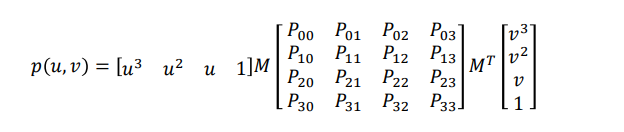
\includegraphics[width=\linewidth]{assets/bezier_patches_point.png}
    \caption{Cálculo de um ponto da superfício, definida com \textit{P} pontos de controlo.}
    \label{fig:bezier_point}
\end{figure}

Assim, segue-se:
\begin{code}
    \captionof{listing}{BezierTriangles}
    \label{code:BezierTriangles.h}
    \inputminted[firstline=5, lastline=15]{cpp}{../../cartesian/BezierTriangles.h}
\end{code}

Para evitar o cálculo constante da matriz de transformação de \textit{Bezier}, $M$, com a matriz dos pontos de controlo da superfície, $P$,
e, consequentemente, o cálculo da resultante, $MxP$, pela transpost, $M^T$, utilizou-se variáveis locais, o que benificia 
no consumo de memória.

\subsubsection{\textit{create\_bezier}}
No âmbito de calcular todas as superfícies criou-se dentro do módulo \textbf{shapes}, 
um método capaz de contruir um objeto, recebendo um vetor com os índices dos pontos de controlo
de cada \textit{patch}, \textit{pacthes},
um vetor com todos os pontos, \textit{points} e o nível de tesselação, \textit{level}.

Deste modo, segue-se:
\begin{code}
    \captionof{listing}{create\_bezier}
    \label{code:shapes.h}
    \inputminted[firstline=44, lastline=44]{cpp}{../../generator/shapes.h}
\end{code}

\subsubsection{Adicional}

A extração de informação encontra-se dentro do módulo \textbf{writer}, na função \textit{main} do \textit{generator},
sendo tudo feito recorrendo ao uso de \textbf{expressões regulares} e da biblioteca \mintinline{cpp}{<regex>}.
\end{document}